\documentclass[10pt,a4paper]{article}
\usepackage[utf8]{inputenc}
\usepackage{amsmath}
\usepackage{amsfonts}
\usepackage{amssymb}
\usepackage{graphicx}
\usepackage[margin=1in]{geometry} 
\usepackage{amsmath,amsthm,amssymb,amsfonts}
 
\newenvironment{problem}[2][Problem]{\begin{trivlist}
\item[\hskip \labelsep {\bfseries #1}\hskip \labelsep {\bfseries #2.}]}{\end{trivlist}}
%If you want to title your bold things something different just make another thing exactly like this but replace "problem" with the name of the thing you want, like theorem or lemma or whatever

\begin{document}
\author{Peter Shaffery}
\title{Numerical Analysis II: Homework 8}
\maketitle
\section{Problems}
\begin{problem}{1}
Determine the order and region of absolute stability for the s-step Adams-Bashforth methods where $s=2,3$.
\end{problem}
\begin{enumerate}
\item When $s=2$ then we have $\rho(w) = w^2 - w$ and $\sigma(w) = \frac{3w-1}{2}$.  We can Taylor expand $\rho(e^w) - w \sigma(e^w) = \frac{5 w^3}{12} + \mathcal{O}(w^4)$, hence the $s=2$ method is second order.  To determine the region of absolute stability we determine for which values of $h \lambda$ the roots of the polynomial in $w$, $\pi(w;h \lambda) = \rho(w) - h \lambda \sigma(w)$, satisfy the root condition $w^* \leq 1$.  This is plotted in Fig. 1a.
\item When $s=3$ then we have that $\rho(e^w) - w \sigma(e^w) = \frac{3 w^4}{8} + \mathcal{0}(w^5)$; calculating the region of absolute stability as above, the result are shown in Fig 1b.
\item The Adams-Moulton method is order 3 and it's region of stability is given in Fig. 1c.
\end{enumerate}

\begin{figure}
\centering
\begin{tabular}{ccc}
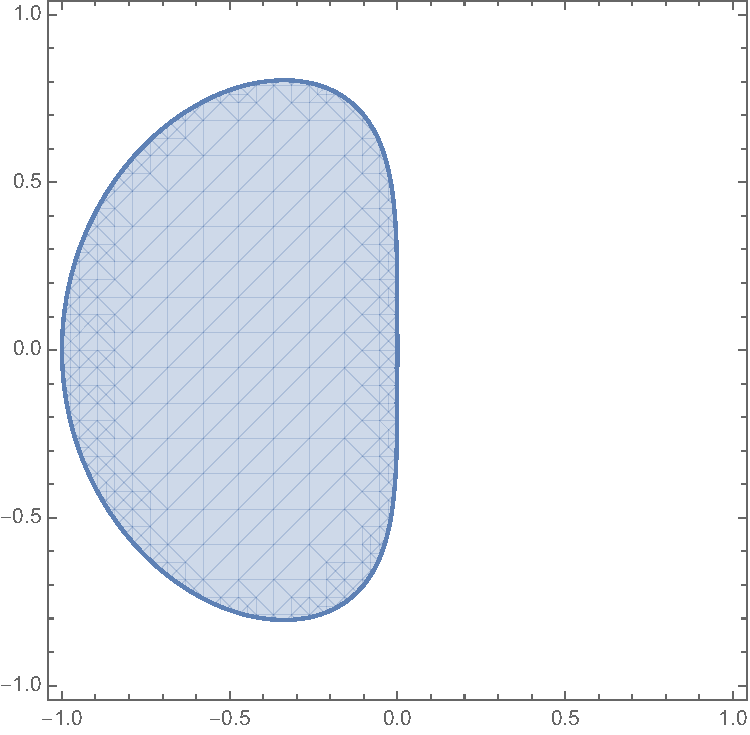
\includegraphics[scale=.3]{./Figs/s2_reg.pdf} & 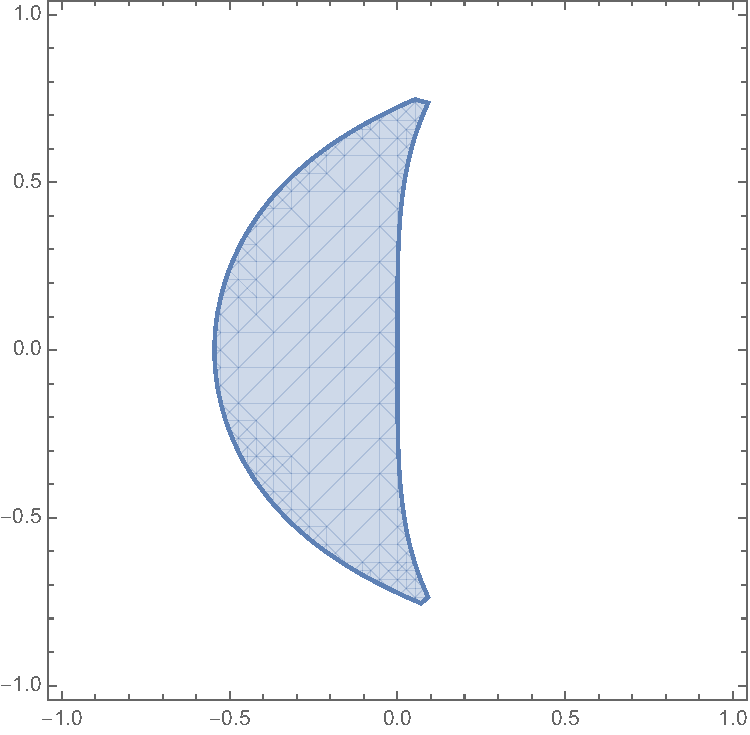
\includegraphics[scale=.3]{./Figs/s3_reg.pdf} & 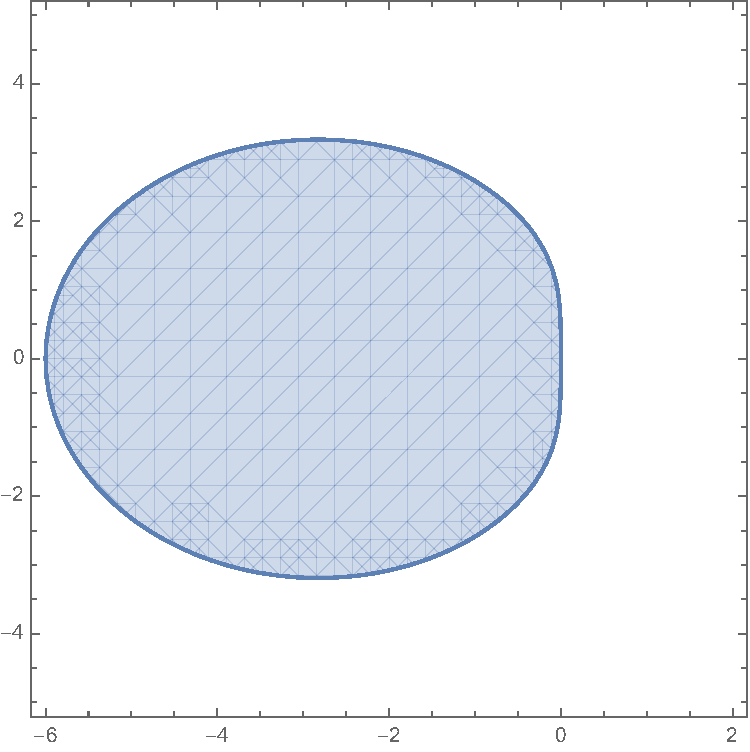
\includegraphics[scale=.3]{./Figs/am_reg.pdf}\\
(a) & (b) & (c) \\
\end{tabular}
\caption{Regions of absolute stability in the complex plane for (a) the two-step and (b) the three-step Adams-Bashforth methods and (c) the two-step Adams-Moulton method.}
\end{figure} 

\begin{problem}{2}
Determine the order and region of absolute stability of the BDF methods of step $s=2,3$.
\end{problem}
\begin{enumerate}
\item Calculated as in problem 1, we have that the BDF method with $s=2$ is of order 2 with region of stability given in Fig. 2a.
\item Similarly the BDF method with $s=3$ is of order 3 with region of stability given in Fig. 2b.
\end{enumerate}

\begin{figure}
\centering
\begin{tabular}{cc}
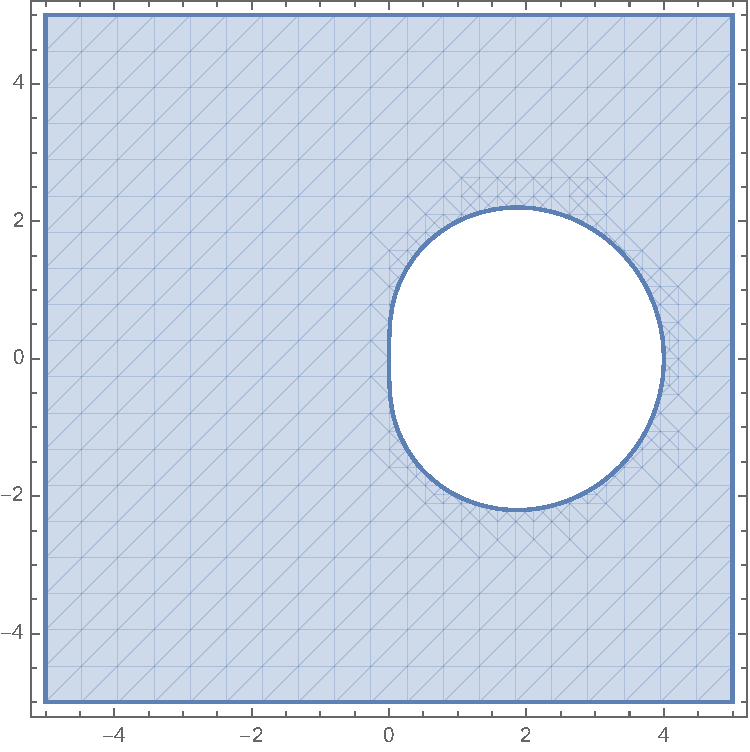
\includegraphics[scale=.3]{./Figs/bdf_s2_reg.pdf} & 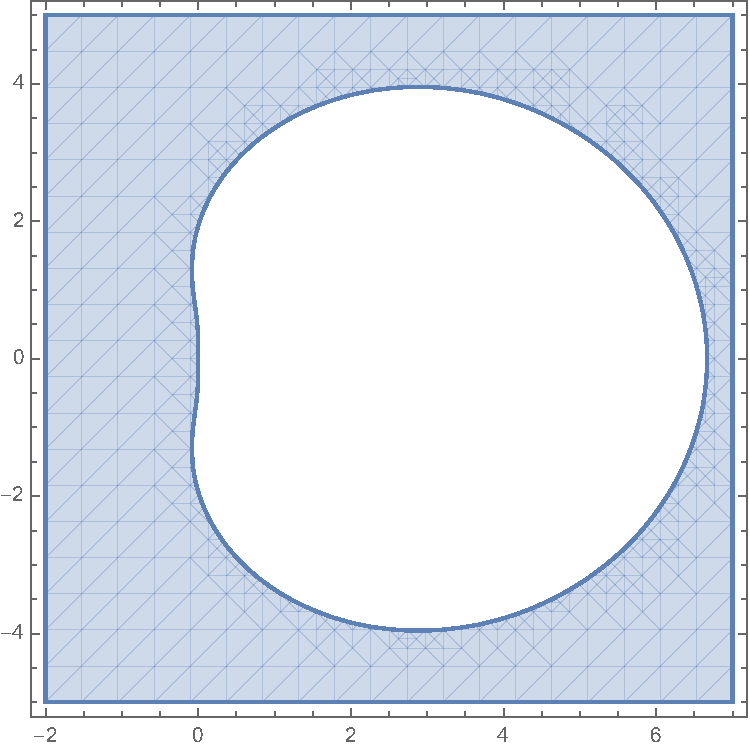
\includegraphics[scale=.3]{./Figs/bdf_s3_reg.pdf} \\
(a) & (b) \\
\end{tabular}
\caption{Regions of absolute stability (shaded blue) in the complex plane for (a) the two-step and (b) the three-step BDF methods.}
\end{figure} 

\begin{problem}{3}
Determine the region of absolute stability of the given Runge-Kutta method.  Calculate all intersections of this region with the real and imaginary axes.
\end{problem}
\begin{proof}
For the test problem $y' = \lambda y$ we have that each step of the RK method is equivalent to $y_{n+1} = \frac{1}{24} [24 + 24 (h \lambda) + 12 (h \lambda)^2 + 4 (h \lambda)^3 + (h \lambda)^4] y_n$, hence finding the region of absolute stability requires determining for which values of $z = h \lambda$ is $\frac{1}{24} (25 + 25 z + 12 z^2 + 4z^3 z^4) < 1$.  We can plot this region in Mathematica without issue (Fig. 3).  

To find the intersection with the real axis we solve $R(z) = \frac{1}{24} (25 + 25 z + 12 z^2 + 4z^3 z^4) = 1$ where $z \in \mathbf{R}$, giving the interval $z \in (-2.79,0)$.  Setting $z = i y$ then we can solve $R(i y) \overline{R(i y)} = 1-\frac{w^6}{72}+\frac{w^8}{576} = 1$ to determine that the intersection is $y \in (-2 \sqrt{2}, 2 \sqrt{2})$.
\end{proof}

\begin{figure}
\centering
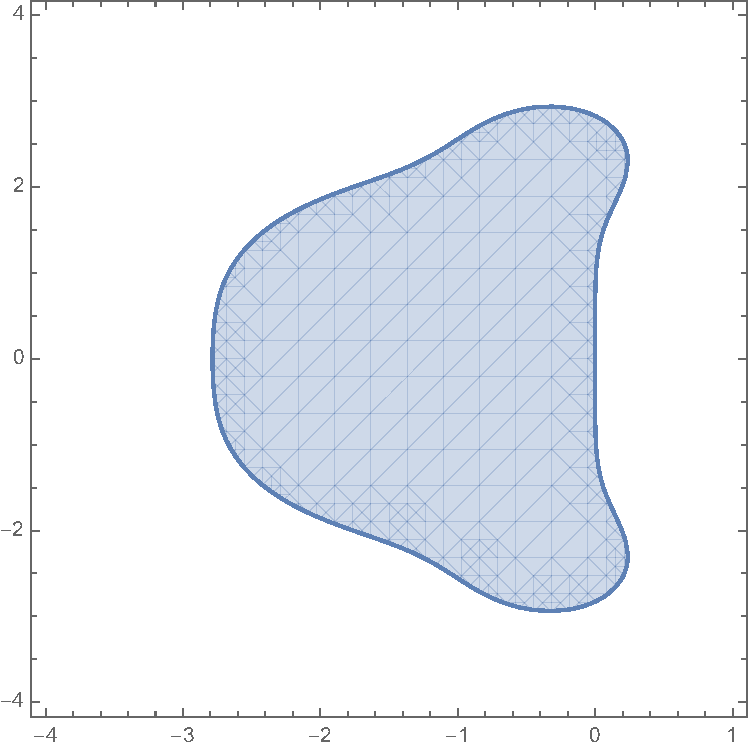
\includegraphics[scale=.4]{./Figs/rk4_reg.pdf}
\caption{Region of absolute stability for the RK4 method}
\end{figure}

\begin{problem}{4}
Given the ODE $\frac{d}{dt} \left[ \left(\frac{1}{1+t} \right) x' \right] + \lambda x = 0$ where $x(0) = 0$, we want to find $\lambda$ such that $x(1) = 0$ using the trap-rule script from a previous assignment.
\end{problem}
Setting $y = x'$ we can convert the ODE to system of coupled DEs:
\begin{equation}
\begin{split}
x' &= y\\
y' &= (1+t)(y - \lambda x)\\
\end{split}
\end{equation}
With IC $x(0) = 0$ and $y(0) = 1$.  Let $\phi_x(\lambda) = x(t=1; \lambda)$ be the flow of this system projected onto $x$, we want to find $\lambda^*$ such that $\phi(\lambda^*) = 0$.  Qualitatively we note that when $\lambda < \lambda^*$ then $\phi_x(\lambda) >0$ and when $\lambda > \lambda^*$ then $\phi_x(\lambda) <0$.  Therefore I'm going to just implement a binary search on the interval $[6.6,6.7]$ (probably due to an error in my implementation of the trap-rule my solutions are all negative for $\lambda \geq 6.7$ so I shifted the given interval).

Doing so gives $\lambda^* = 6.6018303$, see Appendix for code.

\begin{problem}{5}
Consider the boundary value problem $y'' = f(x,y,y')$ for $a < x < b$ where $y(a) = \gamma_1$ and $y(b) = \gamma_2$.
\begin{enumerate}
\item Convert this to an equivalent problem with zero boundary conditions by writing $y(x) = z(x) + w(x)$ with $w(x)$ a straight line statisfying $w(a) = \gamma_1$ and $w(b) = \gamma_2$.  Derive a new BVP for $z(x)$.
\item Generalize this procedure to the same problem with BC $a_0 y(a) - a_1 y'(a) = \gamma_1$ and $b_0 y(b) - b_1 y'(b) = \gamma_2$.  What assumptions, if any, are needed for the coefficients $a_0, a_1, b_0, b_1$?
\end{enumerate}
\end{problem}
\begin{enumerate}
\item Well, right off we have that $w(x) = \gamma_1 + \frac{x-a}{b-a} \gamma_2$, hence $z(x) = y(x) - \gamma_1 - \frac{x-a}{b-a} \gamma_2$.  Therefore $z''(x) = y''(x) + 0 = f(x,y,y'') = f(x,z(x) + \gamma_1 + \frac{x-a}{b-a} \gamma_2, z'(x) + \frac{\gamma_2}{b-a})$ with BC $z(a) = z(b) = 0$.

\item Okay so we still want $y(x) = z(x) + w(x)$ where $w(x)$ is some function that will force $a_0 z(a) - a_1 z'(a)  = b_0 z(b) - b_1 z'(b) = 0$.  Since $y'(x) = z'(x) + w'(x)$ then this is equivalent to force $a_0 w(a) - a_1 w'(a) = \gamma_1$ and $b_0 w(b) - b_1 w'(b) = \gamma_2$.  Can we find a line that satisfies these conditions?  If $w(x) = m x + c$ then:
\begin{equation}
\begin{split}
a_0 m a + a_0 c - a_1 m &= \gamma_1\\
b_0 m b + b_0 c - b_1 m &= \gamma_2\\
\end{split}
\end{equation} 
So as long as $a_i \neq b_i$ for $i = 0,1$ then this gives two equations for two unknowns so there is a unique solution.  I find it in the attached Mathematic script, but to shortcut some obnoxious typesetting let's call them $m^*$ and $c^*$.  Then we can just proceed as we did for Part 1 to plug in $w(x) = m^* x + c^*$ into the original BVP.

\end{enumerate}

\section{Appendix: Code}
\begin{verbatim}
import numpy as np
import scipy as sp
import scipy.optimize as spot
import numpy.linalg as npla
import matplotlib.pyplot as plt
from tqdm import *

class ode_obliterator_v2(dict):
    def __init__(self, RHS, init_val, init_time=0, h=1e-1, q=2,n=2):
        self.yp = RHS
        self.iv = np.array(init_val)
        self.init_time = init_time
        self.t = init_time
        self.h = h
        self.q = q
        self.n = n
        self.dim = max(self.iv.shape)

        self.sol = self.iv
        self.times = np.array([self.t])

    def sacramento_scramble(self,h,curr,t):
        v = curr + .5*h*np.dot(self.yp(t),curr)
        A = np.eye(self.dim) - .5*h*self.yp(t+h)
        output = npla.solve(A,v)
        return(output)

    def basic_trap(self,end,h):
        hold = self.iv
        times = np.arange(self.init_time,end,h)
        curr = self.iv
        for t in times:
            curr = self.sacramento_scramble(h,curr,t)
            hold = np.vstack([hold,curr])
        return(hold)
        
    def boston_u_turn(self,init):
        n = len(init)
        table = np.zeros([n,n])
        table[:,0] = init

        for j in range(1,n):
            for i in range(j,n):
                p = 2*j+1
                table[i,j] = table[i,j-1] +(table[i,j-1] - table[i-1,j-1])/float(self.q**p-1) 

        update = table[n-1,n-1]

        return(update)

    def boulder_shimmy(self,end_time):
        t_steps = np.arange(self.init_time,end_time,self.h)
        self.multigrid = np.zeros([self.n,len(t_steps),self.dim])
        for k in range(0,self.n):
            h = self.q**(-1*k)*self.h
            curr = self.iv
            for t in tqdm(range(len(t_steps))):
                time = t_steps[t]
                for i in np.arange(self.q**k):
                    curr = self.sacramento_scramble(h,curr,time)
                    time += h
                
                self.multigrid[k,t,:] = curr
        
    def houston_plug_n_chug(self,end_time):
        self.boulder_shimmy(end_time)
        hold = np.zeros(self.multigrid.shape[1:3])
        for i in tqdm(range(hold.shape[0])):
            for j in range(hold.shape[1]):
                hold[i,j] = self.boston_u_turn(self.multigrid[:,i,j])

        self.sol = hold
        self.times = np.arange(self.init_time,end_time,self.h)

    
def ode(t,l):
    A = np.array([[0.,1.],[-l*(1.+t),(1.+t)]])
    return(A)

y0 = np.array([0.,1.])
def test(l):
    trap_solve = ode_obliterator_v2(lambda t: ode(t,l),y0, init_time = 0., h = 1e-5,n=2)
    trap_solve.houston_plug_n_chug(1)
    return(trap_solve.sol[-1,0])

#interval = np.array([6.6,6.7])
interval = np.array([ 6.60182937,6.60184])
for index in range(0,5):
    l = np.mean(interval)
    y1 = test(l)

    if y1 < 0.:
        interval = np.array([interval[0],np.mean(interval)])

    if y1 > 0.:
        interval = np.array([np.mean(interval),interval[1]])

    if y1 == 0.:
        break

#okay it's basically lambda = 6.6018303 (after doing some manual tuning like a freaking caveman)
\end{verbatim}

\end{document}

%%% Local Variables:
%%% mode: latex
%%% TeX-master: t
%%% End:
